% Options for packages loaded elsewhere
\PassOptionsToPackage{unicode}{hyperref}
\PassOptionsToPackage{hyphens}{url}
%
\documentclass[
  12pt,
]{article}

% CUSTOM STUFF
% CUSTOM STUFF
% CUSTOM STUFF
% CUSTOM STUFF
% CUSTOM STUFF
% CUSTOM STUFF
% CUSTOM STUFF
% CUSTOM STUFF
% CUSTOM STUFF
% CUSTOM STUFF
% CUSTOM STUFF
% CUSTOM STUFF
% CUSTOM STUFF
% CUSTOM STUFF
% CUSTOM STUFF
% CUSTOM STUFF
% CUSTOM STUFF
% CUSTOM STUFF
% CUSTOM STUFF
% CUSTOM STUFF
\usepackage{multicol}
\usepackage{xcolor}

\definecolor{noteQuoteLine}{RGB}{224,215,188}
\definecolor{noteQuoteBackground}{RGB}{249,245,233}

\newsavebox{\coloredquotationbox}

\newenvironment{noteQuote}
 {%
  \begin{trivlist}
  \begin{lrbox}{\coloredquotationbox}
  \begin{minipage}{\dimexpr\linewidth-2\fboxsep}
 }
 {%
  \end{minipage}
  \end{lrbox}
  \item\relax
  \parbox{\linewidth}{
    \begingroup
    {\color{noteQuoteLine}\hrule}%
    \color{noteQuoteBackground}%
    {\color{noteQuoteLine}\hrule}%
    \endgroup

    \colorbox{noteQuoteBackground}{\usebox{\coloredquotationbox}}\par\nointerlineskip
    
    \begingroup
    {\color{noteQuoteLine}\hrule}%
    \color{noteQuoteBackground}%
    {\color{noteQuoteLine}\hrule}%
    \endgroup
  }
  \end{trivlist}
 }

% CUSTOM STUFF
% CUSTOM STUFF
% CUSTOM STUFF
% CUSTOM STUFF
% CUSTOM STUFF
% CUSTOM STUFF
% CUSTOM STUFF
% CUSTOM STUFF
% CUSTOM STUFF
% CUSTOM STUFF
% CUSTOM STUFF
% CUSTOM STUFF
% CUSTOM STUFF
% CUSTOM STUFF
% CUSTOM STUFF
% CUSTOM STUFF
% CUSTOM STUFF
% CUSTOM STUFF
% CUSTOM STUFF
% CUSTOM STUFF


\usepackage{lmodern}
\usepackage{amssymb,amsmath}
\usepackage{ifxetex,ifluatex}
\ifnum 0\ifxetex 1\fi\ifluatex 1\fi=0 % if pdftex
  \usepackage[T1]{fontenc}
  \usepackage[utf8]{inputenc}
  \usepackage{textcomp} % provide euro and other symbols
\else % if luatex or xetex
  \usepackage{unicode-math}
  \defaultfontfeatures{Scale=MatchLowercase}
  \defaultfontfeatures[\rmfamily]{Ligatures=TeX,Scale=1}
\fi
% Use upquote if available, for straight quotes in verbatim environments
\IfFileExists{upquote.sty}{\usepackage{upquote}}{}
\IfFileExists{microtype.sty}{% use microtype if available
  \usepackage[]{microtype}
  \UseMicrotypeSet[protrusion]{basicmath} % disable protrusion for tt fonts
}{}
\makeatletter
\@ifundefined{KOMAClassName}{% if non-KOMA class
  \IfFileExists{parskip.sty}{%
    \usepackage{parskip}
  }{% else
    \setlength{\parindent}{0pt}
    \setlength{\parskip}{6pt plus 2pt minus 1pt}}
}{% if KOMA class
  \KOMAoptions{parskip=half}}
\makeatother

\IfFileExists{xurl.sty}{\usepackage{xurl}}{} % add URL line breaks if available
\IfFileExists{bookmark.sty}{\usepackage{bookmark}}{\usepackage{hyperref}}
\hypersetup{
  hidelinks,
  pdfcreator={LaTeX via pandoc}}
\urlstyle{same} % disable monospaced font for URLs
\usepackage{listings}
\newcommand{\passthrough}[1]{#1}
\lstset{defaultdialect=[5.3]Lua}
\lstset{defaultdialect=[x86masm]Assembler}
\usepackage{graphicx,grffile}
\makeatletter
\def\maxwidth{\ifdim\Gin@nat@width>\linewidth\linewidth\else\Gin@nat@width\fi}
\def\maxheight{\ifdim\Gin@nat@height>\textheight\textheight\else\Gin@nat@height\fi}
\makeatother
% Scale images if necessary, so that they will not overflow the page
% margins by default, and it is still possible to overwrite the defaults
% using explicit options in \includegraphics[width, height, ...]{}
\setkeys{Gin}{width=\maxwidth,height=\maxheight,keepaspectratio}
% Set default figure placement to htbp
\makeatletter
\def\fps@figure{htbp}
\makeatother
\setlength{\emergencystretch}{3em} % prevent overfull lines
\providecommand{\tightlist}{%
  \setlength{\itemsep}{0pt}\setlength{\parskip}{0pt}}
\setcounter{secnumdepth}{3}
% Make \paragraph and \subparagraph free-standing
\ifx\paragraph\undefined\else
  \let\oldparagraph\paragraph
  \renewcommand{\paragraph}[1]{\oldparagraph{#1}\mbox{}}
\fi
\ifx\subparagraph\undefined\else
  \let\oldsubparagraph\subparagraph
  \renewcommand{\subparagraph}[1]{\oldsubparagraph{#1}\mbox{}}
\fi

\definecolor{listing-background}{HTML}{F7F7F7}
\definecolor{listing-rule}{HTML}{B3B2B3}
\definecolor{listing-numbers}{HTML}{B3B2B3}
\definecolor{listing-text-color}{HTML}{000000}
\definecolor{listing-keyword}{HTML}{435489}
\definecolor{listing-identifier}{HTML}{435489}
\definecolor{listing-string}{HTML}{00999A}
\definecolor{listing-comment}{HTML}{8E8E8E}
\definecolor{listing-javadoc-comment}{HTML}{006CA9}

% \setmonofont{Libertinus Mono}[
%   Scale=MatchLowercase
% ] % or whatever font you prefer



\lstdefinestyle{eisvogel_listing_style}{
  % basicstyle=\footnotesize\ttfamily
  language         = java,
  numbers          = left,
  xleftmargin      = 2.7em,
  framexleftmargin = 2.5em,
  backgroundcolor  = \color{listing-background},
  basicstyle       = \color{listing-text-color}\small\ttfamily{}\linespread{1.15}, % print whole listing small
  breaklines       = true,
  frame            = single,
  framesep         = 0.19em,
  rulecolor        = \color{listing-rule},
  frameround       = ffff,
  tabsize          = 4,
  numberstyle      = \color{listing-numbers},
  aboveskip        = 0.7em,
  belowskip        = 0.1em,
  abovecaptionskip = 0em,
  belowcaptionskip = 1em,
  keywordstyle     = \color{listing-keyword}\bfseries,
  classoffset      = 0,
  sensitive        = true,
  identifierstyle  = \color{listing-identifier},
  commentstyle     = \color{listing-comment},
  morecomment      = [s][\color{listing-javadoc-comment}]{/**}{*/},
  stringstyle      = \color{listing-string},
  showstringspaces = false,
  escapeinside     = {/*@}{@*/}, % Allow LaTeX inside these special comments
  literate         =
  {á}{{\'a}}1 {é}{{\'e}}1 {í}{{\'i}}1 {ó}{{\'o}}1 {ú}{{\'u}}1
  {Á}{{\'A}}1 {É}{{\'E}}1 {Í}{{\'I}}1 {Ó}{{\'O}}1 {Ú}{{\'U}}1
  {à}{{\`a}}1 {è}{{\'e}}1 {ì}{{\`i}}1 {ò}{{\`o}}1 {ù}{{\`u}}1
  {À}{{\`A}}1 {È}{{\'E}}1 {Ì}{{\`I}}1 {Ò}{{\`O}}1 {Ù}{{\`U}}1
  {ä}{{\"a}}1 {ë}{{\"e}}1 {ï}{{\"i}}1 {ö}{{\"o}}1 {ü}{{\"u}}1
  {Ä}{{\"A}}1 {Ë}{{\"E}}1 {Ï}{{\"I}}1 {Ö}{{\"O}}1 {Ü}{{\"U}}1
  {â}{{\^a}}1 {ê}{{\^e}}1 {î}{{\^i}}1 {ô}{{\^o}}1 {û}{{\^u}}1
  {Â}{{\^A}}1 {Ê}{{\^E}}1 {Î}{{\^I}}1 {Ô}{{\^O}}1 {Û}{{\^U}}1
  {œ}{{\oe}}1 {Œ}{{\OE}}1 {æ}{{\ae}}1 {Æ}{{\AE}}1 {ß}{{\ss}}1
  {ç}{{\c c}}1 {Ç}{{\c C}}1 {ø}{{\o}}1 {å}{{\r a}}1 {Å}{{\r A}}1
  {€}{{\EUR}}1 {£}{{\pounds}}1 {«}{{\guillemotleft}}1
  {»}{{\guillemotright}}1 {ñ}{{\~n}}1 {Ñ}{{\~N}}1 {¿}{{?`}}1
  {…}{{\ldots}}1 {≥}{{>=}}1 {≤}{{<=}}1 {„}{{\glqq}}1 {“}{{\grqq}}1
  {”}{{''}}1
}

\lstset{style=eisvogel_listing_style}

\lstdefinelanguage{XML}{
  morestring      = [b]",
  moredelim       = [s][\bfseries\color{listing-keyword}]{<}{\ },
  moredelim       = [s][\bfseries\color{listing-keyword}]{</}{>},
  moredelim       = [l][\bfseries\color{listing-keyword}]{/>},
  moredelim       = [l][\bfseries\color{listing-keyword}]{>},
  morecomment     = [s]{<?}{?>},
  morecomment     = [s]{<!--}{-->},
  commentstyle    = \color{listing-comment},
  stringstyle     = \color{listing-string},
  identifierstyle = \color{listing-identifier}
}

\date{}

\begin{document}







% Front Page begins

\thispagestyle{empty}


%\thisfancyput{%
\begin{center}

%Substitute with the right information
\Large{
\hfill \begin{tabular}{l}
Degree Name \\
Project Module Code \\
ID Number
\end{tabular}
}


%\bigskip
%\bigskip
\vspace*{\fill}

%replace by your Project title
\Large{\textbf{Skeem - a database system to deal with modern needs}}

\vspace*{\fill}

by

\vspace*{\fill}

%Replace by your name

Henry Morgan


%Replace by your supervisor's name
\vspace*{\fill}

Supervisor: Dr. C. Hatter
\vspace*{\fill}

\underline{Department of Computer Science} \\
\underline{Loughborough University}

\vspace*{\fill}
%Delete/Change as appropriate
April/June 2019

\end{center}
%}
\newpage
% Front Page ends




\begin{abstract}
  Skeem is a datbase
\end{abstract}

\newpage













{
\setcounter{tocdepth}{3}
\tableofcontents
}
\newpage
\hypertarget{key-terms}{%
\section{Key Terms}\label{key-terms}}

Key Definitions JSON (Javascript object notation) is a human readable
text format which encodes key-value pairs and arrays of primitive values
(strings, numbers, booleans, nulls). Although JSON technically denotes a
string the term will be also used when referring to a parsed version of
the string i.e JSON may referer to a string denoting an array containing
numbers or an actual instance of an array containing the elements 1,2
and 3.

\hypertarget{introduction}{%
\section{Introduction}\label{introduction}}

This is the introduction Websites are important by 2020 50'000'000
people will have one they take millions of hours to create\ldots. other
facts which emphasis websites

\hypertarget{problem-definition}{%
\section{Problem Definition}\label{problem-definition}}

This chapter will provide an overview of the problem this project will
be attempting to solve. It will provide a high level overview of
existing practices, how they currently function, why they exist and why
they are problems which require solving.

\hypertarget{current-state-of-web-applications}{%
\subsection{Current state of web
applications}\label{current-state-of-web-applications}}

SPAs or single-page applications are a growing trend on the web unlike
traditional architectures where each page is a separate resource with
its own end-point, its own template and its own request, SPAs combine
all the pages into a single end point. When a user navigates to a page
they download a large javascript bundle which has the ability to
construct any page of the website. The javascript is reads the url the
user requested and renders the creates the appropriate views. This means
that when a user navigates to another page, the javascript can intercept
this and simply render new content without a network request creating a
much more responsive interaction.

\begin{noteQuote}

\textbf{Note:} This is a simplified example of how SPAs tend to work. In
reality having a user download the entire code bundle would not be
ideal, especially on slower networks. Therefore optimizations are
performed such as code splitting where the user only downloads the
necessary code to build the requested page and any assets needed to
display loading screens, then during idle time or upon navigation
download any missing code required to render new pages.

\end{noteQuote}

\hypertarget{apis}{%
\subsection{APIs}\label{apis}}

SPAs allow for extremely responsive and interactive websites, however,
they create a new issue - how do you fetch data. Previously the server
was responsible for constructing the page and therefore could query the
database to obtain all the information needed. The client, however, can
not directly query the database and instead must communicate through an
API.

An API accepts requests for specific data and responds in a pre-defined
format. APIs referer to how a system is interacted with, this can
include interactions with code libraries or http interfaces into a
webserver, either way the qualities of a good api are the same. They
provide the ability to request the required data when needed. Good APIs
will consistent, flexible, and specific.

\begin{description}
\tightlist
\item[Consistency]
in an API allows developers to become more familiar with its uses more
quickly and allows them to, correctly, make assumptions about how to use
parts of the API which they previously may not have used. If a developer
has to look at documentation whenever they are attempting something new
then the API may be inconsistent.
\item[Flexible]
APIs do not force developers into pre-determined patterns. APIs should
act to supply the needed data, not determine what data can be shown.
This not only concerns being able to request all data but also being
able to not request unneeded data. For instance, if when a developer
requires an articles title but are forced to receive the entire body of
the article then the end user will be downloading unnecessary data,
which on slower networks could be significant.
\end{description}

Specific :

\begin{lstlisting}[caption={A mock example of an API request and it corresponding response.}]
REQUEST: /api/users
RESPONSE: [ { name: 'Alice' }, { name: 'Bob' }, { name: 'Carol' } ]
\end{lstlisting}

\begin{itemize}
\tightlist
\item
  APIs are hard to make

  \begin{itemize}
  \tightlist
  \item
    Consistent
  \item
    Flexible
  \end{itemize}
\item
  They are either very complicated
\item
  API design usually doesn't require a team of people to maintain but
  everyone needs to interact with at some point, waste of time training
  people
\end{itemize}

\begin{center}\rule{0.5\linewidth}{\linethickness}\end{center}

\begin{itemize}
\tightlist
\item
  Apis tend to require knowledge which is not needed for front end
  development. Another issue with APIs is that they usually require
  knowledge which is not needed for front-end developers. This leads to
  the need for additional training.
\end{itemize}

\begin{center}\rule{0.5\linewidth}{\linethickness}\end{center}

\begin{itemize}
\tightlist
\item
  APIs also tend to be very repetitive i.e you need an end point to
  fetch a list of blogs and you also need one to fetch all the products.
  What is really different about these routes? The table name in the sql
  and the attributes it returns. This duplication of code leads to more
  code which leads to more potential for bugs.

  \begin{itemize}
  \tightlist
  \item
    Lots of code = Lots of bugs.
  \end{itemize}
\end{itemize}

\begin{center}\rule{0.5\linewidth}{\linethickness}\end{center}

Separation of code but a strong connection on functionality.

\begin{itemize}
\tightlist
\item
  SPAs require a server to interact with the database as sql is not safe
  to execute from a client
\end{itemize}

\begin{center}\rule{0.5\linewidth}{\linethickness}\end{center}

\begin{itemize}
\tightlist
\item
  Duplication of requests. Imagine having an end point requesting a list
  of blog posts. On the site you wist to display the title of each blog
  with a short extract from the body to act as a teaser. On this teaser
  you also want to display the authors name. You may also have a author
  page showing information about the author. This leads to an issue of
  either having two end points which return very similar data or reusing
  the end point but then forcing the end user to download more
  information then they actually require.
\end{itemize}

Building an API is easy, building a consistent and flexible API is hard.

\begin{center}\rule{0.5\linewidth}{\linethickness}\end{center}

\hypertarget{authentication}{%
\subsection{Authentication}\label{authentication}}

Not only is it important to be able to request data flexibly but also
limit what data can be accessed per user.

\hypertarget{databases}{%
\subsection{Databases}\label{databases}}

When building any non-trivial database driven application there are
certain features which will need to be implemented.

\begin{itemize}
\item
  Repeated Code

  \begin{itemize}
  \item
    Creating and maintaining a database involves a lot of repeated tasks
  \item
    This server has a lot of code dedicated (sometimes entirely) for
    database interaction.
  \end{itemize}
\item
  Databases are complicated

  \begin{itemize}
  \item
    It requires a lot of understanding to setup and maintain a database
    especially when wanting to perform any non trivial, but abstractly
    simple, tasks such as:

    \begin{itemize}
    \tightlist
    \item
      associations
    \item
      file storage
    \item
      user authentication
    \item
      permissions
    \item
      etc
    \end{itemize}
  \item
    All these tasks are very well defined and understood yet when
    setting up a database you have to reinvent the wheel every time.
  \item
    Many non-technical people could take advantage of a database yet
    don't understand how.

    \begin{itemize}
    \tightlist
    \item
      Think how many excel spreadsheets get used and how complex they
      become
    \item
      People need ordered and relation storage and retrieval systems
    \end{itemize}
  \end{itemize}
\end{itemize}

\begin{center}\rule{0.5\linewidth}{\linethickness}\end{center}

Databases should store normalizes data which, simply speaking means so
structure data in flat tables i.e one for articles, one for authors, one
for comments and then you store relational information on the tables.
E.g a column on the comments table referencing a specific article and an
author field on the article link it to the correct user. This is to
remove duplication and allows database systems to cache and index data
which is the reason databases can be so performant even over enormous
datasets.

The issue with this, however, is that data is not displayed like this to
the end user. The end user is not presented with a page containing an
article and is required to navigate to a separate page displaying the
authors name then have to navigate to a third place to read a list of
comments. Rather the end user will be presented with a single page
containing all the data amalgamated in an easily digestible and pleasant
format. The data the user sees can be envisioned as a tree of data: the
root being the article itself and then containing a connected nodes for
each comment each having further nodes containing their authors.

Requesting a tree of data from a database is an extremely common and
useful thing, however, despite being conceptually simple it can get
incredibly complex even when having to traverse only a few levels deep.

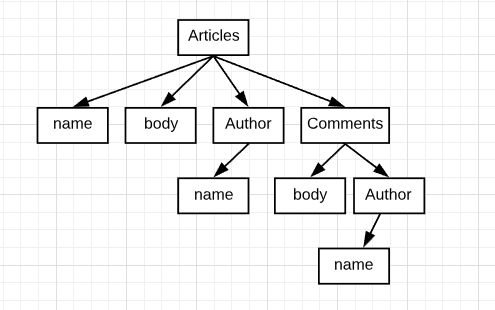
\includegraphics{./images/tree-diagram.png}
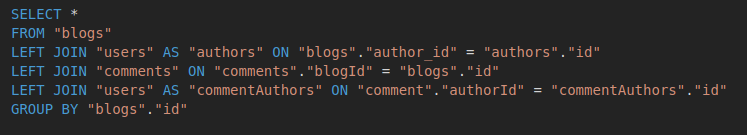
\includegraphics{./images/tree-with-joins.png}

\begin{center}\rule{0.5\linewidth}{\linethickness}\end{center}

\begin{itemize}
\tightlist
\item
  Data consistency

  \begin{itemize}
  \tightlist
  \item
    Once you retrieve the data from a data source (server) it is
    important to keep that up to date
  \item
    if it gets updated on the server it should be reflected on the
    client
  \end{itemize}
\end{itemize}

\hypertarget{literature-review}{%
\section{Literature Review}\label{literature-review}}

In this chapter I shall discuss existing technologies which solve the
defined problem. I shall briefly describe how each solution functions as
well as their advantages and limitations.

\begin{itemize}
\item
  GraphQL + Relay

  \begin{itemize}
  \tightlist
  \item
    Sits on top of an existing
  \item
    Provides a way to query a tree structure of data
  \item
    complicated - non feasible for non technical people
  \end{itemize}
\item
  NoSQL databases

  \begin{itemize}
  \tightlist
  \item
    Stores arbitrarily shaped json allowing data to be stored in a
    fashion similar to its usage
  \item
    eliminates the tree problem
  \end{itemize}
\item
  Web framework

  \begin{itemize}
  \tightlist
  \item
    Rails
  \end{itemize}
\end{itemize}

\hypertarget{requirements}{%
\section{Requirements}\label{requirements}}

\hypertarget{high-level-requirements}{%
\subsection{High level requirements}\label{high-level-requirements}}

\begin{itemize}
\tightlist
\item
  Tree Structures

  \begin{itemize}
  \tightlist
  \item
    Fetch arbitrary tree structures
  \item
    Query interface which is easily sanitizable such that it could be
    executed from even dangerous clients without risk of returning
    non-permitted data.
  \end{itemize}
\item
  Simple:

  \begin{itemize}
  \tightlist
  \item
    Explainable through limited, reasonably sized, help docs
  \item
    Simple GUI interface
  \item
    Requires 0 knowledge of database structures to use associations
  \item
    Includes File management
  \item
    User authentication
  \end{itemize}
\item
  Consistency

  \begin{itemize}
  \tightlist
  \item
    alert clients to changes in data
  \end{itemize}
\end{itemize}

\hypertarget{specification-gathering}{%
\subsection{Specification Gathering}\label{specification-gathering}}

I was given access to a production server

\begin{itemize}
\tightlist
\item
  used by 4'000 unique visitors a day
\item
  4\% are new visitors
\item
  20'000 registered users
\end{itemize}

I went through all interactions with the database and records how it was
being used:

\begin{itemize}
\tightlist
\item
  attributes

  \begin{itemize}
  \tightlist
  \item
    has many through
  \item
    has many through where condition
  \item
    has many with condition
  \item
    has many dependent nullify
  \end{itemize}
\item
  Validations

  \begin{itemize}
  \tightlist
  \item
    presence
  \item
    uniqueness
  \item
    inclusion
  \item
    number greater than
  \item
    uniqueness in scope of attr: value
  \item
    validate uniqueness in scope with condition unless attribute: value
  \item
    Validates on: :create
  \item
    association.attribute must = value
  \item
    validates {[}if/unless{]} attribute: value
  \end{itemize}
\item
  Callbacks

  \begin{itemize}
  \tightlist
  \item
    before\_validation

    \begin{itemize}
    \tightlist
    \item
      default attribute to another attribute if not present
    \item
      default attributes only on create
    \item
      default attributes to parameterized other attribute
    \item
      default attribute to association attribute
    \end{itemize}
  \item
    before\_create

    \begin{itemize}
    \tightlist
    \item
      self.slug = name.parameterize
    \end{itemize}
  \item
    after\_create

    \begin{itemize}
    \tightlist
    \item
      update association
    \item
      send emails
    \item
      update self
    \end{itemize}
  \end{itemize}
\item
  Scopes

  \begin{itemize}
  \tightlist
  \item
    where(attr: value)
  \item
    where.not(attr: value)
  \item
    order(attr: :desc)
  \item
    where association count \textgreater= 1
  \item
    where association count === 0
  \item
    where association attribute
  \item
    where in associations scope e.g where(tag\_id: Tag.published)
  \item
    composing scopes ( adding limits)
  \end{itemize}
\item
  Permissions

  \begin{itemize}
  \tightlist
  \item
    through user association
  \item
    through user association \textbar{} where(attr: value)
  \end{itemize}
\end{itemize}

Using this information I obtained the minimum viable feature set needed

\hypertarget{technical-requirements}{%
\subsection{Technical Requirements}\label{technical-requirements}}

\begin{itemize}
\item
  Create Models

  \begin{itemize}
  \tightlist
  \item
    store basic types strings, number
  \item
    store associations between two models
  \item
    store files
  \end{itemize}
\item
  Fetching

  \begin{itemize}
  \tightlist
  \item
    attributes

    \begin{itemize}
    \tightlist
    \item
      Request primitive attributes such as strings, numbers
    \item
      request associations
    \end{itemize}
  \item
    provide a filter to a query

    \begin{itemize}
    \tightlist
    \item
      request a record given the records id
    \item
      request a record based on its attributes i.e requesting published
      records
    \end{itemize}
  \item
    sort queries

    \begin{itemize}
    \tightlist
    \item
      by attributes
    \item
      by associations attributes
    \end{itemize}
  \item
    pagination queries
  \end{itemize}
\item
  Mutations

  \begin{itemize}
  \tightlist
  \item
    create records
  \item
    Update records
  \item
    delete records
  \item
    add/remove association records
  \item
    upload files
  \item
    validate data
  \end{itemize}
\item
  Sessions

  \begin{itemize}
  \tightlist
  \item
    Authenticate users
  \item
    Specify users permission to access data
  \end{itemize}
\item
  Consistency

  \begin{itemize}
  \tightlist
  \item
    Use web sockets to be alerted to updates
  \end{itemize}
\item
  Permissions

  \begin{itemize}
  \tightlist
  \item
    Specify access (read + write + remove) of users on:

    \begin{itemize}
    \tightlist
    \item
      records
    \item
      attributes
    \end{itemize}
  \end{itemize}
\item
  Provide a way to change production databases safely
\item
  GUI

  \begin{itemize}
  \tightlist
  \item
    Provide a way to create a database
  \item
    Provide a way to create a model
  \item
    add/update/remove attributes from models
  \item
    seed data
  \item
    view records for a model
  \end{itemize}
\end{itemize}

\hypertarget{solution}{%
\section{Solution}\label{solution}}

In order to solve the problem I have created a system named Skeem. Skeem
provides an interface for creating Skeem is designed to be used by
developers. This chapter acts as a high level overview to skeems
functionallity, and how to use it.

\begin{quote}
\begin{itemize}
\tightlist
\item
  What is skeem
\item
  Skeem requires no code
\end{itemize}
\end{quote}

Skeem is a fully manager service Skeem wraps a standard object
relational sql database. It allows queries specifying query trees. It
provides methods to authenticate users and limits their actions. It has
hooks utilizing web sockets to receive updates when ever data changes in
order to prevent a user from viewing stale data. Skeem can be fully
customized and managed from either a command line interface or from a
gui.

\hypertarget{models}{%
\subsection{Models}\label{models}}

Models are one of the most important aspects of Skeem, they define the
data. They control what gets stored and how, as well as how it is
accessed and who can access it. They are akin to database tables but not
neccessarily one to one.

\hypertarget{attributes}{%
\subsubsection{Attributes}\label{attributes}}

At attribute is like a database column, it stores a single piece of data
for a model. Attributes are comprised of a name, a type and a set of
configuration specific the the type chosen.

There are a number of built in attribute types which aim to accomadate
any type of data you may want to store. If, however, you have a need to
store data which one of the built in types do not support then you Skeem
allows for a custom attribute type by the means of a plugin, see the
chapter on {[}attribute plugins{]}{[}{]}

\hypertarget{strings}{%
\paragraph{Strings}\label{strings}}

\begin{itemize}
\tightlist
\item
  presence validations
\end{itemize}

\hypertarget{numbers}{%
\paragraph{Numbers}\label{numbers}}

\hypertarget{booleans}{%
\paragraph{Booleans}\label{booleans}}

\hypertarget{dates}{%
\paragraph{Dates}\label{dates}}

\hypertarget{passwords}{%
\paragraph{Passwords}\label{passwords}}

Password attributes are designed to store Passwords They are distinct
from strings Password attributes can not be retrieved, only updated.
They automatically hash the value supplied to them

\hypertarget{associations}{%
\paragraph{Associations}\label{associations}}

Association attributes store links between models.

\hypertarget{files}{%
\paragraph{Files}\label{files}}

File attributes store

\hypertarget{scopes}{%
\subsubsection{Scopes}\label{scopes}}

Scopes define methods for fetching subsets of data: published articles.
Scopes are built from a tree of comparison functions

\hypertarget{requests}{%
\subsection{Requests}\label{requests}}

Communication with the server is achieved through http requests. This
means that requests can be made from the client. This solves the tight
coupling with disperate code issues between the standard client-server
model.

All requests are fired to the same end point with a post request and
take the form of a JSON object with \passthrough{\lstinline!type!} and
\passthrough{\lstinline!payload!}. The type is used to determine what
type of request it is: fetch, mutate, etc. and the payload contains
specific information depending on the type.

\begin{quote}
TREE OF DATA
\end{quote}

\hypertarget{fetching-data}{%
\subsubsection{Fetching Data}\label{fetching-data}}

Fetching data involves pulling data from the models in a structured
fashion. A fetch query specifies a single root model name as the key to
the query object. The value then specifies exactly what data you want to
retrieve, how to filter and sort it and whether you want to split it
into pages.

A fetch response will always be an array of records, where each record
will contain its own id as well as any additional attributes you
requested. In some cases you may also retrieve the total record count
see the section \protect\hyperlink{pagination}{Pagination}.

\hypertarget{attributes-1}{%
\paragraph{Attributes}\label{attributes-1}}

Attributes specify what data you want to receive for each record.
Attributes take the form of an array where each element is a string
being the name of the attribute you are requesting, or an object with a
name property and a value of the attribute. This object notation is
required for specifying additional configuration such as formatting
information like an alternative name for results.

Attributes can be aliased by specifying the \passthrough{\lstinline!as!}
property

\begin{lstlisting}[caption={This query will return all articles each containing the article’s id, name, and body. The body will be aliased under the name "text"}]
{
  articles: {
    attributes: ["name", { name: "body", as: "text" }]
  }
}
\end{lstlisting}

\begin{quote}
associations: trees of data\ldots..
\end{quote}

\hypertarget{filter}{%
\paragraph{Filter}\label{filter}}

Filters all for specifying specific criteria records must meet for them
to be returned.

Filters you a tree of ``object functions''. This means that each object
within a filter operation contains a single key. This key specifies what
function you which to execute e.g equality, less that, empty check. And
the value acts as the arguments for the given function.

There are many built in filter functions which cover a broad range of
use cases

\hypertarget{sort}{%
\paragraph{Sort}\label{sort}}

Sorting data is an extremely common and essential ability for data
retrieval: Most recent tweets, video length, article title. When sorting
data you specify what you want to sort \passthrough{\lstinline!by!} and
the \passthrough{\lstinline!direction!} you want to sort: either
\emph{asc}ending or \emph{desc}ending.

\begin{lstlisting}[caption={This query will return all articles ordered by the articles "name" attribute.}]
{
  articles: {
    sort: {
      by: "name",
      direction: "asc"
    }
  }
}
\end{lstlisting}

You can also specify an array of sorting criteria. Doing this will sort
the data initially by the first item, then resolve conflicts with the
next item in the list.

\label{pagination}

\hypertarget{pagination}{%
\paragraph{Pagination}\label{pagination}}

Pagination chunks the data into pages. You don't want the end user to
download 100'000 records, this would be very slow and wasteful. The
returned data will be equivalent to a standard array of records.

\begin{lstlisting}[caption={This query will return the second page of articles where each page holds 30 records.}]
{
  articles: {
    pagination: {
      page: 2,
      perPage: 30,
    }
  }
}
\end{lstlisting}

\hypertarget{record-count}{%
\subparagraph{Record count}\label{record-count}}

As well as the actual records, you also get given a count of the number
of records you would have gotten if you did not paginate the data. This
is useful when wanting to show end users a list of page numbers and
allow them to jump to them arbitrarily.

\[ totalPages = ceiling( totalRecords / perPage ) \]

Retrieving the record count can be disabled by passing the option of
\passthrough{\lstinline!withCount: false!} to the pagination block.

\hypertarget{mutating-data}{%
\subsubsection{Mutating Data}\label{mutating-data}}

\hypertarget{permissions-and-security}{%
\subsection{Permissions and Security}\label{permissions-and-security}}

Controlling what users can access, who can create and edit data is an
essential part of all application which make use of a database.

\hypertarget{authentication-1}{%
\subsubsection{Authentication}\label{authentication-1}}

Before we can control a users access we must first be able to determine
who they are. Skeem provides a couple of ways in which to authenticate
someone: stored identifier (email, username, etc) with a password or
through an oauth2.0 provider such as Facebook or Google. These methods
of authentication are referred to generally as session providers (they
provide methods for authentication sessions).

Session provides define a name, model, a type and some configuration
dependant on the type selected.

The name is used purely to distinguish between different providers and
allows for multiple authentication strategies of the same type. You may
have to distinct user sets which are authenticated with different models
e.g for a school system you may have one user set named teachers and
another for pupils. The model defines where the session provider should
look to find the necessary data to check against any credentials
provided.

The type defines which session provider to use. Skeem comes with three
built in providers: local, facebook, and google.

The local provide authenticates users by storing some identifying
attribute and a password in the database itself. Then when an
authentication request is made the database is queried for a record with
the specified credentials. If a record is found then skeem authenticates
the user as that record. The user attribute is most commonly an email
address or a username. The password is stored securely using a secure
hashing algorithm.

The Facebook and Google providers allow users to authenticate using
these services via the familiar ``login with XXX'' buttons. These
providers can specify a list of attributes to extract from the service
such as name, email, image.

\hypertarget{roles}{%
\subsubsection{Roles}\label{roles}}

With authentication we now have two distinct user states: authenticated
and anonymous. These roles can be used to define permissions on fetches
and mutates

\hypertarget{permissions}{%
\subsubsection{Permissions}\label{permissions}}

Each model can define a set of permissions based scopes

\hypertarget{config}{%
\subsection{Config}\label{config}}

Application wide configuration is done by means of a json file named
\passthrough{\lstinline!skeem.json!}

\begin{itemize}
\tightlist
\item
  When running a command the system search recursively upwards from the
  current directory looking for a file named skeem.json
\end{itemize}

TODO

\hypertarget{different-environments}{%
\subsubsection{Different Environments}\label{different-environments}}

Throughout a projects life time it will be run in multiple environements
such as development or production. Each enviroment will likely want its
own configuration. For instance when developing an application you would
want to store files locally for speed and cost, whereas, in production
you problable want to use a cloud storage solution such as AWS.

The configuration for different enviroments can be declared within the
configuration file by nesting all the options within an object and
making the key equal to the name of the environment. Skeem looks at the
\passthrough{\lstinline!NODE\_ENV!} enviroment variable in order to
guage which configuration block should be loaded.
\passthrough{\lstinline!NODE\_ENV!} is a standard variable throughout
the node ecosystem to distinguish between environments.

\begin{lstlisting}[caption={An example of a config with multiple environments.}]
{
  developments: {
    /* development config */
  },
  production: {
    /* development config */
  }
}
\end{lstlisting}

\hypertarget{environment-variables}{%
\subsubsection{Environment Variables}\label{environment-variables}}

There are many settings in skeem for which the value may not want to be
hardcoded. This may be because the value is likely to change often, may
be different for each developer, or because the value should be kept
secret and so would want to avoid be committed into the applications
repository. The solution to that is the use of environment variables.
Environment variables provide run time configuration options to many
programs and are used to solve this issue within skeem.

To use an environment variable you must set the value of the
configuration item to be
\passthrough{\lstinline!\{ $env: 'name of env variable' \}!}. Skeem
searches all values of the configuration for objects in this form and
substitutes them for the specified variable. If this variable does not
exist an error is thrown.

To further facilitate the use of these variables skeem will
automatically search for a file in the application root named ``.env''.
This file should contain key value pairs. Upon starting, skeem will
automatically load this file and merge the contained variables into the
environment prior to passing the configuration.

\begin{lstlisting}[caption={Configuration which uses enviroment variables to avoid exposing critical infomation}]
{
  database: {
    host: { $env: "DATABASE_HOST" },
    username: { $env: "DATABASE_USERNAME" },
    password: { $env: "DATABASE_PASSWORD" },
  },
}
\end{lstlisting}

\hypertarget{errors}{%
\subsection{Errors}\label{errors}}

There are many aspects of skeem which could result in errors

\begin{multicols}{2}
\begin{itemize}
\item missingCordToken
\item invalidToken
\item malformedRequest
\item malformedFileRequest
\item modelNotFound
\item tableNotFound
\item unknownAttributes
\item unknownScope
\item unknownScopeFunction
\item malformedScopeQuery
\item noModifyId
\item recordNotFound
\item fileNotFound
\item validation
\item uncastable
\item argumentError
\item unsortableAttributeType
\item providerNotFound
\item missingSessionCredentials
\item placeholderError
\item server
\item internal
\item internalUnknownProviderType
\item internalUnknownAttributeType
\item internalUnknownValidationType
\item internalMissingParamSchema
\item invalidAuthToken
\item internalProviderNotFound
\item unknownMigrationChangeType
\item invalidMigrationChangeData
\item unknownRole
\item configError
\item four04
\item typeError
\item noSchemaFound
\item tooManySchemas
\item providerNotSpecified
\item providerNotConfigured
\item providerNoOAuth
\item providerNoDirectionAuth
\item scopeAlreadyExists
\item migrationValidation
\item clientArgumentError
\item malformedLoginRequest
\item fileHandlerConfiguration
\item nonReversible
\item runningMigrationsAbort
\item rollbackMigrationsAbort
\item roleAlreadyExists
\item privateModel
\item permissionDenied
\item invalidCustomAttribute
\item parsingMigration
\item dbNotUpToDate
\item configForEnvDoesntExist
\item configMissingPath
\item liveNotConfigured
\item unknownSeedHandler
\item seedingError
\item unknownCallbackType
\item noGetterForAttribute
\item noSetterForAttribute
\item invalidFilter
\item invalidCustomOperator
\item invalidCustomSessionProvider
\end{itemize}
\end{multicols}

\hypertarget{management}{%
\subsection{Management}\label{management}}

There are two predominant methods to managing a skeem application:
through the use of a command line interface or via a GUI.

The first step in using skeem is to initialize a project. The easiest
way to do this is to use Skeems command line interface (CLI). The CLI
has a lot of functionality to help you manage your database and
configure your application, see (\#CLI). To initialize the project
simply run the command \passthrough{\lstinline!skeem init myProject!}.
This will create all the necessary files and folders in the current
directory for an application named ``myProject''. The next step would be
to create a model.

\hypertarget{cli}{%
\subsubsection{CLI}\label{cli}}

\hypertarget{gui}{%
\subsubsection{GUI}\label{gui}}

\hypertarget{the-client}{%
\subsection{The Client}\label{the-client}}

Skeem has a client, written in Javascript, designed to be used with
SPAs. The client provides functions which will process queries and send
them to the server.

\hypertarget{caching}{%
\subsubsection{Caching}\label{caching}}

\hypertarget{validations}{%
\subsubsection{Validations}\label{validations}}

\hypertarget{oauth-flows}{%
\subsubsection{Oauth flows}\label{oauth-flows}}

\hypertarget{live-updates}{%
\subsection{Live Updates}\label{live-updates}}

\hypertarget{plugins}{%
\subsection{Plugins}\label{plugins}}

APIs are a large and complex systems which cover an increadly broad
range of use cases. It would be almost impossible to foresee every use
case of skeem and to allow for every possibility. As such, skeem has the
ability to augment functionality by the way of plugins.

Plugins are javascript files located in the project folder. When the
server starts these files are loaded, type checked, and inserted into
the system.

\hypertarget{custom-attributes}{%
\subsubsection{Custom attributes}\label{custom-attributes}}

There are many different types of datum which you may want to use which
don't fit within the bounds of the built in types.

The attributes built in to skeem use this very system i.e they contain
no special functionality which could not be implemented outside of the
core code.

\hypertarget{custom-session-providers}{%
\subsubsection{Custom session
providers}\label{custom-session-providers}}

There are many different ways you may want a user to authenticate.

\hypertarget{custom-operation-functions}{%
\subsubsection{Custom operation
functions}\label{custom-operation-functions}}

There are a myriad of different and obscure filters you may want to
perform within a database. Whilst skeem contains alot of built in
operations which can achieve a large variety of results it is
implausible that they cover every possible desire.

Therefore, like with attributes, skeem provides the ability to create
custom operation function outside of the skeem source and have them
loaded in dynamically and used seamlessly with the built-in operations.

\hypertarget{creating-an-operation}{%
\paragraph{Creating an operation}\label{creating-an-operation}}

An operation consists of a single function which must return SQL.

\begin{lstlisting}[caption={The simplist custom operation - it would always return false and so is utterly pointless.}]
function myPointlessOperation() {
  return { value: `'this will' = 'always be false'` }
}
\end{lstlisting}

In order to create a useful operation the function is passed some
variables concerning the request. The most useful of which is the
\passthrough{\lstinline!value!} argument. The
\passthrough{\lstinline!value!} contains the data passed to the
operation. Using this we can produce a much more useful operation.

\begin{quote}
The SQL returned is inserted into the query as is and so is essential
that it is sanitied prior to being returned.
\end{quote}

\begin{lstlisting}[caption={Returns all the records for which the name matches the value supplied. However there are major issues with this and should not be used.}]
function myBadOperation({ value }) {
  return { value: `"name" = '${value}'` }
}
\end{lstlisting}

The above operation shown in figure (FIGURE XXX) would technically do
something which could be deemed as useful. You supply is a value and it
will return all the results for which their name attribute is equal to
that value. There are a couple of issues with this operation though
which means it should not be used.

The biggest and most critical issue is that it does not sanitize the
value. This means it is an entry point of an SQL injection. This is
relatively easy to solve though through the use of a sister package of
skeem named es-qu-el. That is outside the scope of this solution chapter
and is discussed in the implementation.

The second issue with the operation is that it makes the assumtion that
the model you are currently fetching has a column in its table called
``name''. This is not always true for obvious reasons. To solve this
issue we are passed another useful piece of infomation - the current
model. With this we can search through the models attributes and check
for the existance of a name attribute and if it does exist then throw an
error.

This is an extremely common need for skeem and as such there exists a
helper function to achieve this for you. It os exported from the
\passthrough{\lstinline!skeem-common!} package and is called
\passthrough{\lstinline!getAttribute!}. This function takes a model and
the name of the attribute you wish to retrieve. By using this function
you guarantee that the attribute exists and if it does not exists then
you can be assured that you will get an error message consistent with
that of a built in error.

\begin{lstlisting}[caption={Checks to see if name actually exists on the model being queried.}]
const { getAttribute } = require("skeem-common")

function mySlightlyBetterOperation({ model, value }) {
  const attribute = getAttribute(model, "name")
  return { value: `"${attribute.name}" = '${value}'` }
}
\end{lstlisting}

There is one final issue with this operation and that is it misses the
opportunity for optimization. As well as returning the SQL value
operations can also return the type of result expected back from the SQL
- in this case it would be a ``boolean''. Supplying this infomation from
an operation allows Skeem to optimize the SQL query and possibly not
even execute anything. For instance consider the following query:

\begin{lstlisting}
{
  filter: {
    eq: [{ value: "a string" }, { value: 123 }]
  }
}
\end{lstlisting}

The \passthrough{\lstinline!value!} operation will return the types of
string and number (as well as the sanitized SQL value). The
\passthrough{\lstinline!eq!} operation then checks these types to see if
they are save it is then it will place the values around an equals sign
and return it as expected. If, however, they are different then the
\passthrough{\lstinline!eq!} operation will return with a type of
``false''. If the full filter resolves with the type of ``false'' skeem
will skip executing the query as it knows nothing would be returned.
Therefore by returning the correct type skeem can potentailly optimize
and avoid the database altogether.

Possible types include:

\begin{itemize}
\tightlist
\item
  string
\item
  boolean
\item
  number
\item
  record
\item
  collection
\item
  any - the type could not be determined and so could be anything, this
  is the default when no type is returned
\end{itemize}

\begin{lstlisting}[caption={Checks to see if the attribute actually exists and returns the correct type}]
const { getAttribute } = require("skeem-common")

function myPassableOperation({ model, value }) {
  const attribute = getAttribute(model, "name")
  return { value: `"${attribute.name}" = '${value}'`, type: "boolean" }
}
\end{lstlisting}

It should also be noted that this is a poor use of a custom operation.
This operation does not achieve anything that you could not do with the
built in operations. Although it does save a few characters, it adds on
additional knowledge needed by other people working on a project, the
need for testing, and another function which would need maintaining over
the life time of the project. Operations should only be added to achieve
results which are either not possible with the pre-existing functions or
highly impracticle to achieve.

\hypertarget{nested-operations}{%
\paragraph{Nested operations}\label{nested-operations}}

It is very common for an operation to need to accept an operation object
as its value. If you could not compile nested operations then you would
not be able to create functions like: \passthrough{\lstinline!eq!},
\passthrough{\lstinline!lt!}, \passthrough{\lstinline!and!},
\passthrough{\lstinline!not!}. This would make things a little tricky.
Therefore, along with model and query you also get supplied with a
function named \passthrough{\lstinline!compile!}. This function accepts
an operation and returns the \passthrough{\lstinline!\{value, type\}!}
object.

\begin{lstlisting}[caption={A simple implementation of the eq operaion.}]
const { getAttribute } = require("skeem-common")

function simpleEq({ compile, value }) {
  const left = compile(value[0])
  const right = compile(value[1])
  return { value: `${left.value} = ${right.value}`, type: "boolean" }
}
\end{lstlisting}

\hypertarget{the-request-context}{%
\paragraph{The request context}\label{the-request-context}}

the final argument passed to an operation is
\passthrough{\lstinline!ctx!}. This is the current context for the
request. With this it is possible to access infomation such as app
configuration, the current session, and the database connection.

TODO

\hypertarget{using-an-operation-plugin}{%
\paragraph{Using an operation plugin}\label{using-an-operation-plugin}}

To use an operation you first must create a javascript file within the
\passthrough{\lstinline!<skeem root>/operations!}. The name of this file
does not matter and can be anything. This javascript file must have a
default export of an object where the keys are the names of the
operations and their values are the functions as described above.

\begin{lstlisting}[caption={A full operation plugin file}]

module.exports = {
  isANumber: function({ value }) {
    if (typeof value === 'number') {
      return { value: true, type: 'boolean' }
    } else {
      return { value: false, type: 'boolean' }
    }
  }
}

// Usage:

fetch:   {
  articles: {
    filter: {
      { isANumber: 123 }
    }
  }
}
\end{lstlisting}

\hypertarget{documentation}{%
\subsection{Documentation}\label{documentation}}

Documetnation exists for skeem which contains guides and examples on how
to use the system. This is essential to allow other developers to
actually use the system. \url{https://cd2.github.io/Skeem/\#/}

\hypertarget{methodology}{%
\section{Methodology}\label{methodology}}

\hypertarget{development-strategy}{%
\subsection{Development Strategy}\label{development-strategy}}

When a new feature would be added it would first have high level tests
written aimed to test the final functionallity of the feature. For
instance when first implementing fetching I wrote tests asserting that
given a particular query a specific piece of sql was generated. I would
then proceed to implement the feature, using the tests as a guide for
when the work was complete.

\begin{lstlisting}[caption={Example of what the high level tests would assert (not actual tests)}]
Given: { articles: {} }
Expected: `SELECT "id" FROM "articles"`

Given: { articles: { attributes: ["name"], filter: { eq: [ { attr: 'name' }, {value: 'test'}] } } }
Expected: `SELECT "id", "name" FROM "articles" WHERE "attr" = 'test'`
\end{lstlisting}

Once all the tests were passing, if there were additional features which
either appeared during implementation or that were initially excluded
for simplicity, I would add more high level tests asserting the new
functionallity. I would then proceed to implement these features until
the new tests were passing, adding more tests until development was
complete.

When the feature was complete, assert by a suite of passing tests I
would begin testing the code at a more granular level. I would select
functions which were either complicated or hard to test at a high level
(maybe code branches for very specific circumstances) and write specific
unit tests.

The specifics of how the tests are written are discussed more in the
chapter (Testing){[}\#testing{]}.

\hypertarget{implementation}{%
\section{Implementation}\label{implementation}}

In this chapter I shall be explaining some of the intricacies of skeem,
how it works, and why certain key decesicions have been made. This
chapter will not cover the implementation of everything skeem offers but
instead covers a the key aspects for which their were challanges and
interesting solutions.

\hypertarget{technologies}{%
\subsection{Technologies}\label{technologies}}

\hypertarget{typescript}{%
\subsubsection{Typescript}\label{typescript}}

Some parts of Skeem runs on the client side and thus had to be built in
javascript.

Typescript is a superset of javascript which adds typing capabilities to
the normally dynamic language ({\textbf{???}}). This typing infomation
allows compile time code checking which greatly assists improving
relaibility of code as it helps to ensure against common trivial bugs.
Typescript is transpiled into standard, es5 compliant, javascript
meaning it is able to run on all modern browsers. This compatibility is
essential because if skeem only supported the latest version of chrome
then it would instantly elliminate the possibility of using the system
on any standard website which has compatibility as a requirement.

Typescript also aids other developers using the system as the typing
infomation is used in most modern IDEs to supply intellisence infomation
allow features such as auto completion, inline errors messages, and
hints for expected arguments and returns.

NodeJs is a javascript runtime designed to build scalable network
application ({\textbf{???}}). NodeJs was a logical choice as it allowed
writing server code also in javascript which allowed consistent
interfaces to be constructed. It is also much easier to develop a system
when writing in a single language as their is less mental energy exerted
to convert from one environment to another.

\hypertarget{postgres}{%
\subsubsection{Postgres}\label{postgres}}

Postgres is a object-relational database system ({\textbf{???}}).
Postgres has powerful, inbuilt JSON processing capabilities. It allows
for storing JSON objects natively as well as writing queries which
inspect the contents of JSON. More importantly Postgres allows for the
construction of JSON objects with queries themselves. This makes
Postgres a very logical choice when the goal is to create trees of data
as the database can pre-format the response greatly reducing the need
for much post query processing.

Another feature which postgres offers is an optimizer which can
automatically transform subqueries into join statements. This
optimzation is greatly taken advantage of in skeem as throughout the
code base there is not a single joining statement. Further reasons for
this are discussed in the chapter on fetch query sql generation.

Postgres also provides the ability to write custom database functions
relatively easily. These functions help to encapsulate complex pieces of
reusable logic and are optimized by postgres in order to maintain
performant queries. They are used in a number of place throughtout skeem
such as to trigger update messages for live syncing and to format
responses in certain circumstances.

\hypertarget{other-libraries-and-services}{%
\subsubsection{Other Libraries and
Services}\label{other-libraries-and-services}}

Skeem also takes advantage of a number of prebuilt libraries and
services.

\begin{description}
\tightlist
\item[NPM]
NPM is the defacto package manager for node ({\textbf{???}}), it
provides easy hosting and distribution of node packages and is the
method skeem uses to manage its publications.
\item[Pusher]
Pusher is a web service specialised in providing real-time functionality
to applications ({\textbf{???}}). It provides simple wrappers are web
sockets as well as fallbacks to ensure compatibility accross, even
outdated, browsers. Skeem uses Pusher send messages to clients in order
to enable the live updating capabilities.
\item[Amazon Web Services]
AWS is a cloud computing platform({\textbf{???}}) which provides
relatively affordable file hosting and is integrated into skeems file
storage capabilities.
\item[React]
React
\end{description}

\begin{quote}
TODO
\end{quote}

\hypertarget{project-structure}{%
\subsection{Project Structure}\label{project-structure}}

Due to the size of the skeem code base (pushing 12'000 lines) and the
range of environments it runs on (server and the client). It was
essential to split up the project into logical parts. However I did not
want to fully isolate each section due to the tight coupling of the
interactions e.g if the format of the fetch response changes then you
have to update the server code to handle this new change as well as the
client code to keep the format consistent from a developers point of
view. Due to this I structured the code as a monorepo.

\begin{quote}
``A monorepo is a software development strategy where code for many
projects are stored in the same repository'' (``Monorepo'' 2019).
\end{quote}

Then using a tool named Lerna I was able to manage the projects
simultaneously. Lerna automatically resolves the dependency order so,
for instance, when you attempt to build the project it knows that A
depends on B which depends on C and therefore wait for A to build before
moving on to B then finishing with C.

Skeem is broken up into 7 packages, 5 directly related packages, each
prefixed with ``skeem-'', specific to skeem and 2 auxilary packages
which were extracted and can provide useful functionallity
independently:

\hypertarget{skeem-server}{%
\subsubsection{skeem-server}\label{skeem-server}}

This package contains the majority of the logic, it contains the
implemention for processing requests, creating a database, session
authentication, migration creating and validation, etc\ldots{}

The \passthrough{\lstinline!skeem-server!} package is split into two,
confusingly named, parts: a manager and a server. The manager contains
the all the functionallity of the app, it controls loading the schema,
producing and executing SQL, updating config, etc. The server simply
listens for http requests sent from the client, performs basic format
type checking and then calls manager functions in order to create a
response.

\hypertarget{server}{%
\subsubsection{Server}\label{server}}

\hypertarget{manager}{%
\subsubsection{Manager}\label{manager}}

\hypertarget{skeem-cil}{%
\subsubsection{skeem-cil}\label{skeem-cil}}

This implements a command line interface for interacting with skeem, it
implements no fundamental logic and instead acts a wrapper around the
server.

\hypertarget{skeem-gui}{%
\subsubsection{skeem-gui}\label{skeem-gui}}

Similar to the CLI, the gui acts a wrapper around the server
functionality and displays the information in a visual application.

\hypertarget{skeem-client}{%
\subsubsection{skeem-client}\label{skeem-client}}

Provides functionallity for a client

\hypertarget{skeem-common}{%
\subsubsection{skeem-common}\label{skeem-common}}

Holds common functionallity needed between packages, such as error
messages

\hypertarget{es-qu-el}{%
\subsubsection{es-qu-el}\label{es-qu-el}}

provides helper functions to generate and sanitize SQL statements

\hypertarget{typer}{%
\subsubsection{Typer}\label{typer}}

Typer standardies type checking accross the app.

\hypertarget{overseer}{%
\subsubsection{overseer}\label{overseer}}

declarative CLI generator used to power Skeems CLI.

\hypertarget{database-management}{%
\subsection{Database Management}\label{database-management}}

\hypertarget{skeem--tables}{%
\subsubsection{skeem-* Tables}\label{skeem--tables}}

Skeem relies on a handful of datebase tables in order to function. Each
of these tables are prefixed with ``skeem-'' in order to differentiate
them from application specific tables.

\begin{description}
\tightlist
\item[skeem-schema]
Stores the applications schema
\end{description}

skeem-migrations :Stores a list of all migrations

skeem-sessions :stores a list of sessions, including what record the
session was for, when the session was created, when the last activity
for the user occurred and what session provider was used to
authenticate.

skeem-images :stores references for files uploaded to Skeem

skeem-version :stores the current database version

\hypertarget{functions}{%
\subsubsection{Functions}\label{functions}}

Skeem also relies on a few custom functions in order to properly handle
certain requests.

\hypertarget{upgrading-the-database}{%
\subsubsection{Upgrading the Database}\label{upgrading-the-database}}

In order to accomadate new functionalitty it is likely the features of
the database may have to change, new tables may be required, old tables
may need to columns, etc. In order to facility this need skeem provides
a database upgrade mechanism.

This upgrade system works by keeping track of a database version number
and a list of steps on how to upgrade from one version to another. When
the server is started the current version number is loaded from the
database and compared to the most highest upgrade number available. If
these are equal the database is fully up to data and the system proceeds
as normal. If however they are different the database goes through the
update process.

The update process involves iterating through all upgrade steps starting
from the current version number counting up until all steps have been
executed. After each step the version number is updated in order to keep
it in sync with the database state allowing for the possibility of an
error within the upgrade step.

As of the time of writing there are 6 upgrade stages (starting from 0).
These stages perform the following:

\begin{enumerate}
\def\labelenumi{\arabic{enumi}.}
\setcounter{enumi}{-1}
\tightlist
\item
  Check to see if the database exists, if it does not the attempt to
  create it.
\item
  Install neccessary extensions, setup tables, initialize empty schema.
\item
  Rename tables from ``cord-\emph{" to "skeem-}'' (The project under
  went a renaming to prevent conflicts with previous systems) and add
  columns \passthrough{\lstinline!exectued!} and
  \passthrough{\lstinline!timestamp!} to the migrations table.
\item
  updating the schema format to accomadate some new features.
\item
  Create response formatting functions to remove inconsistencies of
  certain edge case requests.
\item
  Add a \passthrough{\lstinline!loggedOut!} column to the sessions
  table. previously sessions were deleted.
\end{enumerate}

When creating a new application the version number would attempt to be
loaded but an error would be thrown as no database would exist. This
error is caught and the version number is deemed to be -1. This means
that when creating a new application by simply starting the server a
database will be created automatically (as step 0 would execute). This
greatly improves the time to setup and start using a Skeem application.

\hypertarget{schema}{%
\subsection{Schema}\label{schema}}

\begin{itemize}
\tightlist
\item
  Every application has a single schema
\item
  The schema is responsible for defining all aspects of the site from
  how and what data is stored to how people can authenticate and what
  information different people can access
\end{itemize}

The schema is a single large JSON object which holds infomation
concering all aspects of the application. When an application is first
created its schema is initialized to an empty skeleton.

The schema is stored in the database in the table ``skeem-schema''. This
table only ever holds a single row. When the schema is updated the table
is cleared and the new schema is inserted.

The schema is serializable.

\begin{lstlisting}[caption={The empty schema}]
 {
  db: {
    functions: [],
    tables: []
  },
  models: [],
  providers: []
}
\end{lstlisting}

The schema has three top level keys, db, models, and providers.

\passthrough{\lstinline!db!} holds infomation about the database. This
includes a record of all tables including their name, columns indexes,
and constraints. It also stores a list of custom defined functions.

\passthrough{\lstinline!models!} stores all the models created within
the application.

\passthrough{\lstinline!providers!} holds infomation about the available
session providers. Each provider contains a name, its type as well as
specific configuration for the given provider type.

\hypertarget{models-1}{%
\subsection{Models}\label{models-1}}

Each model has an assocated table

\begin{itemize}
\tightlist
\item
  Always has an id
\end{itemize}

\hypertarget{attributes-2}{%
\subsection{Attributes}\label{attributes-2}}

Attributes have a get, set, and migrate method.

\hypertarget{built-in-attributes}{%
\subsection{Built in attributes}\label{built-in-attributes}}

Skeem supplies a number of built in attributes. These attributes hope to
cover the majority of use cases and also act to demonstrate the
capabilities of the attributes system in order to act as guides for
other developers implementing their own attributes via the plugin
system.

\hypertarget{strings-1}{%
\subsubsection{Strings}\label{strings-1}}

asdasdsa strings are always TEXT columns. Postgres internally stores
text, varchar and char columns in the same underlying datastructure.
This means there is no performance difference between each type. TEXT
was chosen as it has no limit on length nor the need to specify one.
https://www.postgresql.org/docs/9.1/datatype-character.html. They always
default to an empty string and can never be null. This was done to
create consistency accross an application as if an end-user is presented
with an input box then they can never enter a null even if they do not
enter anything it will be an empty string. This means there is a
distinction between attributes which once appeared within a form and
ones which did not. Therefore strings are never null.

\hypertarget{migrate}{%
\paragraph{Migrate}\label{migrate}}

\hypertarget{get}{%
\paragraph{Get}\label{get}}

The get method for strings is very simple.

\hypertarget{numbers-1}{%
\subsubsection{Numbers}\label{numbers-1}}

\begin{itemize}
\item
  numbers are numeric or integers depending on the config.
\item
  passwords are TEXT
\item
  dates are timestamps without timezones
\item
  booleans: are booleans and always default to false
\item
  associations: store links between models. assocations go in a single
  direction. associations are always stored in with a joining table even
  if the association is a one-to-one or a one-to-many. Traditionally you
  would store the assocated record id within the table it self and only
  have a joining table for a many-to-many out of necessity. This was
  done because it means assocations can be transformed from a one to a
  many without the need for complex resolution steps involving creating
  a new table and then cloneing the data from the on-table column.
\item
  file attributes: purely exist with in the schema i.e nothing changes
  about the database when a file field is added or removed. files are
  stored out of the database and a reference is inserted into the
  ``skeem-images'' table. This table stores a reference string used to
  retrive the file, as well as what model the image is for and the id of
  the record it relates to within that model.
\end{itemize}

\hypertarget{migrations}{%
\subsection{Migrations}\label{migrations}}

Migrations are the way the schema is mutated. They provide a simple and
reversible method for manipulation.

\begin{itemize}
\item
  Migrations work to mutate the schema
\item
  They allow multiple developers to work on a single application
\item
  A record of all changes made to the database
\item
  Migrations serve incremental, reversible changes to the schema
\item
  Migrations are stored in files within a folder named migrations
  located in the root of a skeem project
\item
  This allows for migrations to be transferred between computers
\item
  only stored in files to transfer computers, the ones which get
  executed are actually stored in the datbaase
\end{itemize}

\hypertarget{database-diffing}{%
\subsubsection{Database Diffing}\label{database-diffing}}

After a new schema has been produced for an application, a list of
change steps must be realised in order to mutate the existing database.
This happens are migrations are run or when the application is
initialized. In the latter case the empty schema is used as the old
schema.

The first step of this process is to compare the new schema and the old
one in order to find what is actually different. Because the models and
providers only exist in the abstract, as opposed to the db property
which is backed by database tables, only the db of the schema is diffed.

The first step in diffing the dbs is to isolate which tables are new,
which have been removed and which have been \textbf{potentially}
updated. The name field of the table is used to link the old and the new
schema. If a name exists in the old schema but not in the new, then the
table is marked as deleted. Similarrly if a name exists in the new
schema but not the old it is marked as created. If the name exists in
both then the table is marked as potentially updated and undergoes a
further diff.

For each new table the appropriate
\passthrough{\lstinline!CREATE TABLE!} SQL query is generated and
appended to a list of all pending database queries. Like wise for each
removed table a \passthrough{\lstinline!DROP TABLE!} query is produced
and appended to the list.

For each updated table each column

The list of sql commands is then executed. To do this, first, a new
transaction is created within the database. This means if an error
occurrs within the mutate steps the database can be fully restored to
prior to the mutations. Without this then the schema could become out of
sync with the database. The list of sql statements is the run
sequentially. After each step has been executed the schema in the
databse is replaced by the new schema. Finally, a commit message is sent
to postgres informing it to proceed with the mutations. By updating the
schema within the same transaction ensures syncricity between the tables
and the schema.

\hypertarget{requests-1}{%
\subsection{Requests}\label{requests-1}}

All requests to the skeem server are a post request sent to the same end
point. Request bodies are JSON objects which contain two keys:
\passthrough{\lstinline!type!} and \passthrough{\lstinline!data!}.

There is a second format request bodies can take - multipart data.
Multipart requests are designed to effectiently transfer large data
objects such as files and are designated by the content type of
\passthrough{\lstinline!multipart/form-data!}. Skeem expects multipart
bodies to contain a single data field named
\passthrough{\lstinline!body!}. This body should be a JSON string which
contains all the data normally present in a standard JSON request. The
rest of the body contains file data which is processed and exposed to
skeem via the requests context. The body field is extracted and treated
as the main body and processing the request continues as normal.

\begin{quote}
Note: if more then one data field is detected, or the body field is
missing, or the body field is not valid JSON then the a malformed
request error is thrown and the request aborted.
\end{quote}

The \passthrough{\lstinline!type!} part of the body is used to route the
request to an apprioriate handler.

If an error is detected with a requests body at any point, either during
the inital routing of the request or later after delegating by the type,
a malformed request error will be thrown.

Responses always take the form of a JSON object with two keys: error and
data - this is similar to stdout and stderror.

If an error is throw during a request it is first caught then it is
checked against a list of known skeem errors (skeem errors consitently
have a type and a data where the type is one of a limited number of
errors). If it is a skeem error then the response error property is set
this error and the request is ended. If it is not then a new Skeem error
is created of type server (the list specific type of error).

\begin{quote}
If the system is in the development environment then the error will have
the stack trace appended to it to aid debugging.
\end{quote}

\hypertarget{fetches}{%
\subsection{Fetches}\label{fetches}}

All fetch requests perform a single database request independent of how
simple or complex of a query is made. This is a major reason as to why
skeem is so performant.

Fetches start by performing some basic type assertions about the
incoming request. The request is checked to be an object with a single
key. This key is ensured to be a valid model name and that this
modelName actually exists. The value of the object is ensured to be an
object with some subset of the keys: filter, attributes, sort,
pagination. If there are any additional keys the request is deemed to be
errorneous. If any of the checks fail then a malformed request error is
thrown containing additional infomation explaining the exact issue.

\begin{lstlisting}[caption={A malformed request and the corrosponding response}]
REQUEST:
{ articles: {},  comments: {} }

RESPONSE:
{ data: undefined, error: { type: 'malformedRequest', data: 'multiple models passed to fetch query. only one allowed.' }
\end{lstlisting}

The fetch request constructs an object name
\passthrough{\lstinline!SqlQuery!}. This object holds all the infomation
about the final query to be executed, such as the current columns being
selected, the where conditions, the limit etc\ldots{} Each step in
processing a fetch request simply adds additional infomation to this
object.

After the type assertions are complete and the SQL object is
instantiated the next stage is to process the filter and permissions.
This is dont first as there is a chance the filter may conclude that no
results could be returned - in this case the request can be prematurely
aborted and there was no time wasted in processing features like the
attributes.

A filter is simply an operation function

After compiling a filter the attributes are processed. Attributes define
precisly what data is returned. if no attributes are specified within
the fetch query then only the id is returned.

Attributes take the form of an array (this is asserted by a type check)
this array contains either strings or objects. If an element is a string
then it is inflated becoming
\passthrough{\lstinline!\{ name: "the string value" \}!}. This creates
an array of object each with a name property. The name property on the
attributes relates to directly to an attribute on the model. This is
looked up and an error is thrown if the attribute is not found. The
attributes get method is then called allowing attributes to fully
control what it means to retrieve an attribute.

\begin{lstlisting}[caption={The algorithm used to parse the attributes part of a fetch query}]
For each attribute query in the array
  if the attribute query is a string then
    inflate it to become { name: "attribute query string value" }
  end

  find the attributeSchema for the given model whose name matches the attribute queries name property.

  if the attribute doesnt exist then
    throw an unknown attribute type error
  else
    call the attributes get method passing it the attribute query object and the select statement.
  end if
end for
\end{lstlisting}

Sorting is applied next\ldots\ldots\ldots.

Finally pagination is applied - the simplest of all the steps. Like the
other steps the pagniation request is type checked to be an object with
the keys of \passthrough{\lstinline!perPage!},
\passthrough{\lstinline!page!}, and an optional key of
\passthrough{\lstinline!withCount!}. \passthrough{\lstinline!page!} and
\passthrough{\lstinline!perPage!} are numbers and the
\passthrough{\lstinline!withCount!} a boolean.

The query limit is then set to be the value of
\passthrough{\lstinline!perPage!}, and an offset is calculated from
\passthrough{\lstinline!page!} and \passthrough{\lstinline!perPage!} and
applied. If the \passthrough{\lstinline!withCount!} option is excluded
of set to true then a flag is set on the query to include the count in
the final result. This flag is discussed in more depth in the following
chapter on SQL Generation.

\[ offset = (page - 1) * perPage \]

\hypertarget{sql-generation}{%
\subsubsection{SQL Generation}\label{sql-generation}}

After processing is done the query object must be transformed into SQL.
This object is specific to the fetch query and formats its response such
that it can be returned without any post processing.

\begin{lstlisting}[caption={Example logic within the SqlQuery to create the final query}]
SELECT ${columns specified joined by ","}
FROM ${table name}
WHERE ${conditions specified joined by " AND "}
\end{lstlisting}

TOOD:

\hypertarget{the-withcount-flag}{%
\paragraph{The withCount flag}\label{the-withcount-flag}}

If the \passthrough{\lstinline!withCount!} flag is specified then skeem
\ldots.. TODO

\hypertarget{mutations}{%
\subsection{Mutations}\label{mutations}}

\hypertarget{sessions}{%
\subsection{Sessions}\label{sessions}}

\hypertarget{authentication-2}{%
\subsubsection{Authentication}\label{authentication-2}}

\begin{enumerate}
\def\labelenumi{\arabic{enumi}.}
\item
  type check request
\item
\end{enumerate}

\hypertarget{cli-1}{%
\subsection{CLI}\label{cli-1}}

\begin{itemize}
\tightlist
\item
  The cli interacts with skeem by means of a text based command line.The
  was split into an actual definition of the interface and the parsing
  and processing of the command line text.
\item
  Command Definition:

  \begin{itemize}
  \tightlist
  \item
    Commands are defined declaratively as an object containing: a name,
    some help text, a list of accepted options and arguments (each with
    a name, a type and an optional default) and a function to call when
    the command is executed. Skeem currently contains 14 commands.
  \end{itemize}
\end{itemize}

\begin{figure}
\centering
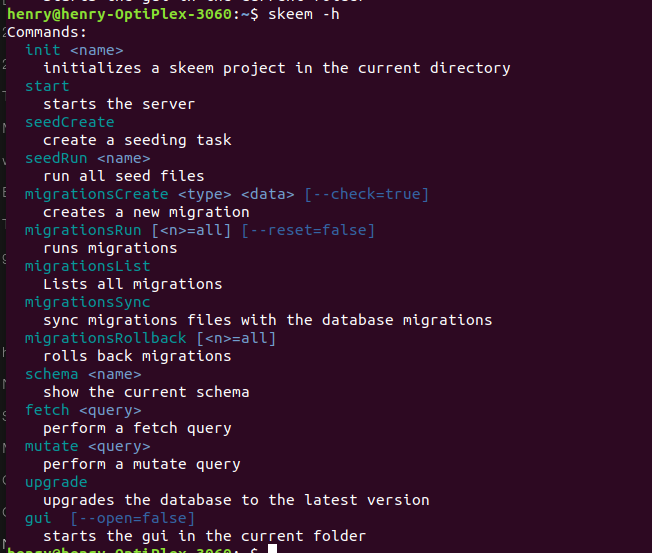
\includegraphics{./images/cli-help.png}
\caption{CLI Help screen}
\end{figure}

\hypertarget{overseer-1}{%
\subsubsection{Overseer}\label{overseer-1}}

\hypertarget{plugins-1}{%
\subsection{Plugins}\label{plugins-1}}

Plugins allow skeem to cover a much wider use case then would likely be
possible if I had to implement all edge cases manually. They also
provide a way to prevent the core of skeem to become bloated with
extremely specific features.

\begin{quote}
Note: There are examples of very specific features within the code base
such as the \passthrough{\lstinline!associationEquals!} operation. It
was, in fact, the addition of features such as this which prompted the
need for the plugin system.
\end{quote}

Every pluggable feature (attributes, session proviers, operators and
file handlers) all work off the same abstracted code and each one simply
specifies a set of configuration. The abstracted code handles the file
loading and parsing and exposes key functions to the specific
implementations.

Each pluggable feature specifies the following:

\begin{description}
\tightlist
\item[name]
this is used when logging debug information.
\item[builtinsFolder]
this specify the name of the folder where the built in features can be
located.
\item[folderName]
the folder name of where the external plugins will be located relative
to the application root.
\item[validateExports]
a function which will get passed a file when it has been imported and
parsed. This function should return a boolean indicating whether the
exported contents of the file is valid. For instance checking whether a
file handler contains a store and retrieve method.
\item[merge]
a function responsible for merging all the individual files together
into one final object.
\end{description}

Abstracting the plugin system like this helped to enforce a consistent
plugin style (which can aid developers when writing plugins), reduce
duplicated complexity, and to isolate a critical system feature to be
tested separately.

\begin{lstlisting}[caption={The code required to define the attribute plugin system}]
export const loadAttributes = createPluginLoader<IAttribute>({
  name: "attributes",
  builtinsFolder: "./builtins",
  folderName: CUSTOM_ATTRIBUTES_PATH,
  validateExports(_filename, exps) {
    // attributes should be an object with three keys: "migrate", "get", "set"

    if (!isObject(exps)) {
      return false
    }

    const expectedKeys = ["migrate", "get", "set"]
    const isValid = Object.keys(exps).every(key => expectedKeys.includes(key))
    return isValid
  },
  merge(acc, filename, exps) {
    acc[filename] = exps
    return acc
  }
})
\end{lstlisting}

Loading a plugin executes the following algorithm:

\begin{enumerate}
\def\labelenumi{\arabic{enumi}.}
\tightlist
\item
  combine the \passthrough{\lstinline!builtinsFolder!} variable and the
  directory the function was defined in, in order to find the full path
  for the built ins.
\item
  if this path doesnt exist, then skip steps 2-6.
\item
  load a list of all files in this directory.
\item
  for each javascript file require it
\item
  pass the contents to the validateExports method along with the file
  name. If this function returns false, throw an error
\item
  otherwise, store the contents along with the file name in an array.
\item
  combine the \passthrough{\lstinline!folderName!} variable and skeems
  root directory to gain a full path for where external elements are
  stored.
\item
  repeat steps 2-6 using this new path.
\item
  for each element in the loaded array, pass it to the merge function.
\item
  return the result of the merge.
\end{enumerate}

When skeem is started it calls all the loaded functions created by the
plugin system. These functions will then load all the built elements and
any external ones, merge them, and then store them with the manager.
Then when a component wants to use one of the plugagble elements it
references it through the manager.

\label{testing}

\hypertarget{testing}{%
\section{Testing}\label{testing}}

Tests are an essential part of any software project especially those
providing some critical functionallity to users - Skeem is no exception.

Tests were written in Jest.

\begin{itemize}
\tightlist
\item
  Tests were written in jest.
\item
  Tests targeted functionality rather then implementation. However tests
  were written for smaller parts of the system when functionality became
  too complex or when the underlying functions were critical - such as
  loading the schema from the database.
\item
  For a complete list of all tests please see the apendix.
\item
  CI

  \begin{itemize}
  \tightlist
  \item
    Due to skeem being used in production it was essential that it was
    not only tested but that testing was constantly carried out. By
    using CircleCI tests are automatically run when a change deployed to
    the git repository.
  \end{itemize}
\item
  Coverage

  \begin{itemize}
  \tightlist
  \item
    Code coverage reports show how many lines of the are touched by the
    tests this is very useful to ensure all the code branches are tested
    and perform as expected.
  \item
    Code coverage ended up at 46\% at the end of the project.
  \end{itemize}
\item
  Code quality

  \begin{itemize}
  \tightlist
  \item
    Codeclimate is a service which analyzes code and detects ``code
    smells''. ``A code smell is any characteristic in the source code of
    a program that possibly indicates a deeper problem.'' - Wikipedia.
    This includes problems such as:

    \begin{itemize}
    \tightlist
    \item
      Cognitive complexity: how complicated is the code to understand.
    \item
      File and function length: does the file or function contain too
      many lines (only counting actual lines of code, ie. not comments
      or blank lines)
    \item
      Duplication: are large parts of the code duplicated in multiple
      places
    \end{itemize}
  \item
    Codeclimate then predicts the amount of time it would take to fix
    this technical debt. At the project end, skeem contained 147 code
    smells with a predicted clean up time of 2 months.
  \end{itemize}
\end{itemize}

\hypertarget{deployments}{%
\section{Deployments}\label{deployments}}

\begin{itemize}
\tightlist
\item
  Throughout the development i has the opportunity to deploy skeem on
  real world applications. At this point skeem is in production use in
  two apps and in employed on 3 further, currently in development,
  projects.
\item
  Resooma

  \begin{itemize}
  \tightlist
  \item
    Resooma is a bills consolidation company focussing primarily on
    university students.
  \item
    88 distinct models, 700 attributes, 50'000'000 users
  \end{itemize}
\item
  Quote generator and Stock management tool for Enterprise Security
  Distributions Norwich

  \begin{itemize}
  \tightlist
  \item
    Tracks more than XXX quotes for customers concerning more than
    20'000 products. Used heavily
  \end{itemize}
\item
  II

  \begin{itemize}
  \tightlist
  \item
    Invoice fraud detection using machine learning
  \end{itemize}
\item
  Voluble

  \begin{itemize}
  \tightlist
  \item
    Messages API
  \end{itemize}
\item
  Rolecall

  \begin{itemize}
  \tightlist
  \item
    Job tracking and communication platform aimed at contract workers
  \end{itemize}
\end{itemize}

There are a wide range of projects using skeem. Very flexible.

\hypertarget{conclusion}{%
\section{Conclusion}\label{conclusion}}

Skeem has turned out to be a very successfull project already helping
out a wide range of projects

\hypertarget{future-work}{%
\subsection{Future Work}\label{future-work}}

\newpage

\hypertarget{references}{%
\section*{References}\label{references}}
\addcontentsline{toc}{section}{References}

\hypertarget{refs}{}
\leavevmode\hypertarget{ref-monorepo_definition}{}%
``Monorepo.'' 2019. \emph{Wikipedia}. Wikimedia Foundation.
\url{https://en.wikipedia.org/wiki/Monorepo}.


\end{document}
